\documentclass[border=6pt]{standalone}
\usepackage{tikz}
\usetikzlibrary{arrows.meta,positioning}
\begin{document}
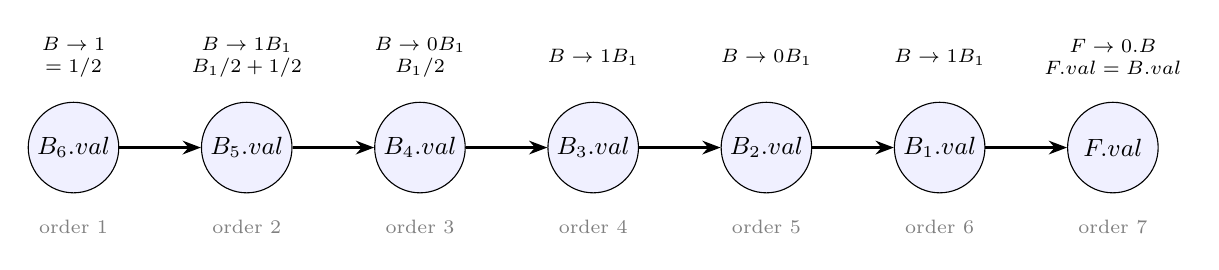
\begin{tikzpicture}[>=Stealth,font=\small,
 n/.style={draw,circle,minimum size=1.15cm,inner sep=0pt,fill=blue!6}]
\node[n] (b6) at (0,0) {$B_6.val$};
\node[n] (b5) at (2.2,0) {$B_5.val$};
\node[n] (b4) at (4.4,0) {$B_4.val$};
\node[n] (b3) at (6.6,0) {$B_3.val$};
\node[n] (b2) at (8.8,0) {$B_2.val$};
\node[n] (b1) at (11,0) {$B_1.val$};
\node[n] (f)  at (13.2,0) {$F.val$};
\foreach \a/\b in {b6/b5,b5/b4,b4/b3,b3/b2,b2/b1,b1/f} \draw[->,thick] (\a) -- (\b);
\foreach \x/\k in {0/1,2.2/2,4.4/3,6.6/4,8.8/5,11/6,13.2/7}
  \node[font=\scriptsize,gray] at (\x,-1) {order \k};
\node[font=\scriptsize,align=center] at (0,1.15) {$B\to 1$\\$=1/2$};
\node[font=\scriptsize,align=center] at (2.2,1.15) {$B\to 1B_1$\\$B_1/2+1/2$};
\node[font=\scriptsize,align=center] at (4.4,1.15) {$B\to 0B_1$\\$B_1/2$};
\node[font=\scriptsize,align=center] at (6.6,1.15) {$B\to 1B_1$};
\node[font=\scriptsize,align=center] at (8.8,1.15) {$B\to 0B_1$};
\node[font=\scriptsize,align=center] at (11,1.15) {$B\to 1B_1$};
\node[font=\scriptsize,align=center] at (13.2,1.15) {$F\to 0.B$\\$F.val=B.val$};
\end{tikzpicture}
\end{document}
